\section{Replication crisis and meta-analysis}

In the 60s and 70s, there was a conflict in clinical psychology. On
one side were the Freudians, protective of the practice of psychodynamic
therapy, a therapy based on concepts such as the unconscious and the
importance of early life experiences. On the other side were the behaviourists,
who mocked Freud's theory as unscientific, and preferred their variant
of therapy, one that didn't need to postulate the existence of unobservables
such as the unconscious \parencite[Chapter 4]{wampold_basics_2010}. It
was against this backdrop the first meta-analysis was done. \cite{smith_meta-analysis_1977}
collected all available high-quality evidence on the efficacy of psychotherapies.
They used statistical methods to integrate all of it into a whole.
The main conclusions of this meta-analysis are still held to be true:
1.) Psychotherapy is an effective treatment and, 2.) there is no difference
in effectiveness between different schools of therapy, the so-called
\emph{Dodo bird verdict.}

The meta-analysis' competitor is the\emph{ narrative review}, where
the author uses her own expertise to amalgamate all the evidence she
is aware of. The meta-analysis is preferred to a narrative review
since it has a greater objectivity. A narrative review gives the author
ample freedom to choose which studies to include, how to weigh the
different studies, what questions or ideas to focus on and how to
frame the results. In addition, a narrative review has no built-in
safeguards against the biases of the author -- this allows for \emph{motivated
reasoning }\parencite{Kunda1990-ry}, which could severely impact
the quality of the review. On the other hand, a properly conducted
meta-analysis allows for fewer of these choices. One reason for this
is how meta-analysis deals with the protocols for collecting data
and conducting analyses, as they should be registered beforehand \parencite{Egger1997-ue};
another is the transparency and replicability of the analysis. Meta-analyses
does not allow idiosyncratic choices of how to frame problems, as
statistical estimates are in focus. While a narrative review tells
a story about a research fields, a meta-analysis gives you dry, numerical
quantities such as $\widehat{\mu}$ and $\widehat{s}$, quantities
that should represent the most current, most objective estimates of
the effect size and its standard error. As such, the meta-analysis
has been called the\emph{ platinum standard of evidence}, playing
on the claim that randomized controlled trials represent the gold
standard of evidence \parencite{Stegenga2011-zo}.

But there is another, more practical reason to prefer meta-analyses
over narrative reviews. When faced with studies numbering a hundred
or more, it is a daunting task for any researcher to process the information
in all of them without aid. The methods of meta-analysis allows the
researcher to process such ``big data'' without suffering from information
overload. Some data is especially difficulty to interpret and work
with, for instance heterogeneous data, data with covariates, or the
otherwise non-standard data. \parencite[][p. 2]{borenstein_introduction_2009}

Since the primary results of a meta-analysis are statistics and $p$-values,
the results can be interpreted in the same detached way as you would
interpret individual studies. And the practical consequences of amalgamating
evidence in this way can be dramatic. It can well be that all the
published studies on a treatment are inconclusive, with effect sizes
going in opposing directions and all $p$-values greater than $0.05$,
but a meta-analysis of the exact same studies is definitive, demonstrating
a positive effect without reasonable doubt. An example is the meta-analysis
of \cite{cannon_meta-analysis_2006} on the effect on heart attack
prevention of high-dose statin therapy compared to standard-dose statin
therapy. The meta-analysis covers four studies, where only one has
a significant $p$-value. Still, the meta-analysis obtains a highly
significant ($p<0.0001$) effect in the desired direction of better
response to higher doses. 
\begin{figure}[h]
\noindent \begin{centering}
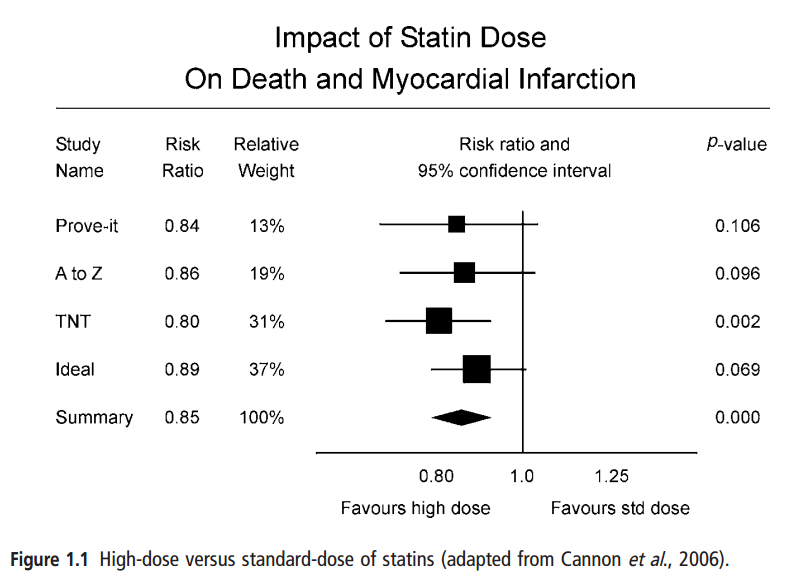
\includegraphics[scale=0.5]{chunks/cannonetal2006}
\par\end{centering}
\caption{\label{fig:A-forest-plot}A \emph{forest plot} of the studies included
in \cite{cannon_meta-analysis_2006} meta-analysis on statins. The
table is from \cite[p. 4]{borenstein_introduction_2009}.}
\end{figure}

Despite being terribly important, often the difference between life
and death\footnote{See the preface of \cite{borenstein_introduction_2009} for a story
of how earlier adoption of meta-analyses could have saved the lives
of thousands of babies that suffered from sudden infant death syndrome.}, meta-analyses have two weaknesses. The first weakness is subjectivity.
For while a meta-analysis is by nature less subjective than a narrative
review, it might still be too subjective to settle a scientific question
once and for all. This problem is emphasized by \cite{Stegenga2011-zo},
and is exemplified by the continuing meta-analysis wars in the research
on the effect of violent video games on aggressive behavior, as discussed
by \cite{elson_twenty-five_2014}. The other weakness are systematic
biases that are hard to model. One of these biases is \emph{publication
bias}, the tendency to publish only positive results. The other is
\emph{p}-hacking, the phenomenon where researchers unconsciously manipulate
studies to get small \emph{p}-values.

\subsection{The problems of meta-analysis}

There is a certain degree of subjectivity in any data analysis, and
the greater leeway to make subjective choices, the stronger the tendency
for the authors to make self-serving choices. An extreme variant of
this is covered by \cite{steegen_increasing_2016}, where it was
shown that a study about the combined effect of relationship status
and fertility could be analyzed in at least 210 different ways. Only
some of these gave results in the desired direction and, not surprisingly,
the published paper had results in the desired direction as well. 

The meta-analyst must choose which studies to include in her meta-analysis.
There is often a good deal of subjectivity here, for it is rarely
so that a study is unambiguously eligible for inclusion. There are
many reasons to exclude a potential study from a meta-analysis. An
oft-discussed bias is \emph{location bias}. If the meta-analysts
are English, they will have a hard time incorporating foreign language
studies into their meta-analysis \parencite{Egger1998-kj}, resulting
in a location-specific meta-analysis. In addition, the meta-analyst
will often include only studies from peer-reviewed scientific journals,
ignoring studies from dissertations or the gray literature. There
are trade-offs involved in the choice of including non-published studies.
On one hand, inclusion of unpublished studies might reduce publication
bias \parencite{Egger1997-ue},
but it could also increase the bias of the meta-analysis. The reason
is that the meta-analyst must rely on her network of researchers to
obtain the unpublished studies -- but her network is likely to be
biased in exactly the same direction as she is. An example of this
effect is found in \cite{ferguson_much_2010}'s discussion of \cite{anderson_violent_2010}'s
meta-analysis on the effect of violent video games on behaviour. The
literature on video game violence and aggression is divided into two
camps. The camp associated with Anderson holds that violent video
games cause aggression, the camp associated with Ferguson holds that
they do not. In order for a meta-analysis to be accepted by all camps,
it should not be biased against including studies from the opposite
camp. However, \cite{anderson_violent_2010} included several unpublished
studies in their meta-analysis, but all were from their own Anderson's
group or associated groups. Ferguson and Kilburn 
\begin{quote}
For example, of two unpublished studies, both are from Anderson et
al.\textquoteright s broader research group. Of three in-press manuscripts
included, two (67\%) are from the Anderson et al. group. Of conference
presentations included, 9 of 12 (75\%) are from the Anderson et al.
group and colleagues. 
\begin{flushright}
-- \cite[p. 2]{ferguson_much_2010}
\par\end{flushright}

\end{quote}
Another source of subjectivity is whether to only include randomized
controlled trials. There is broad agreement that only randomized controlled
trials should be included in a meta-analysis if these trials exists
\parencite{Egger1997-ue}. The reason is that randomized
controlled trials are not affected by confounders in the same ways
as e.g. case control studies and other observational studies. However,
excluding observational studies violates the principle of total evidence,
that your conclusions should be based on all available evidence, not
just a subset of it, see \cite{Stegenga2011-zo} for an extended
discussion.

A reason to exclude a study is that it does not fulfill a list of
best practices. Not all studies are created equal, some are simply
of better quality than others. For instance, a subset of studies might
have much better measuring instruments than the rest, making it reasonable
to include only the studies with the good measuring instrument. But
this is yet another source of subjectivity. As an example \parencite[taken from][p. 6]{lakens_reproducibility_2016},
consider the following ``best-practice'' from \cite{anderson_violent_2010}'s
aforementioned meta-analysis on the effect of violent video games
on behaviour. In order to qualify for a best-practice study, the control
group must be exposed to a non-violent game, while the treatment group
must be exposed to a violent game. One unaccepted treatment-control
pair was \emph{Mortal Kombat} vs \emph{Sonic the Hedgehog.} While
Mortal Kombat is a fighting game infamous for its violence, Sonic
the Hedgehog involves playing a hedgehog jumping on robots, and would
easily be classified as among the least violent games by many researchers.
On the other hand, an accepted treatment-control pair was \emph{Simpsons
Hit \& Run }vs \emph{Grand Theft Auto 3, }even though Simpsons Hit
\& Run involves pulling people out of their car in high-speed situations. 

Finally, studies can be excluded since they look suspicious. There
are many cases of both reporting errors \parencite{nuijten_prevalence_2016}
and downright fraud in the research literature, with Diedrik Stapel
being a high-profile fraudster from social psychology. Since research
data is seldom available, the meta-analyst will not be able to check
the veracity of the reported results in each research paper. This
can lead to exclusion of studies on seemingly ad-hoc grounds. As an
example, take \citeauthor{ferguson_angry_2015}'s 2015 meta-analysis
on the effect of violent video games on aggressive behaviour. In this
analysis, he excluded the study of \cite{gentile_effects_2009} due
to what \cite{ferguson_angry_2015} called ``bouncing beta'' regression
coefficients, or regression coefficients of equal magnitude going
in opposite directions. For a response to this claim, see \cite{gentile_what_2015}'s
rejoinder.

\subsubsection{Choice of statistical technique}

After the meta-analyst is done collecting her data, she must chose
how to analyze them. Now she is faced with two categories of models,
namely the class of \emph{fixed effect models} and \emph{random effects
models} \parencite[chapter 10]{borenstein_introduction_2009}. In order
to explain these models, I will need some technical notation. So let
$N(\mu,\sigma)$ denote the normal distribution with mean $\mu$ and
variance $\sigma^{2}$, and allow $z_{i}$ to be the estimated effect
size of the $i$th study. Under this simple set up, the fixed effects
model works under the assumption $z_{i}\sim N(\mu,\sigma_{i}n_{i}^{-1/2})$.
The pith of this model is that all studies are assumed to \emph{exactly
equal}. On the face of it, this is an unacceptably unrealistic assumption.
Still, the model will often be the best choice, mostly due to the\emph{
bias-variance trade-off} \parencite[p. 37]{friedman_elements_2001}. Since
our data is imprecise, it is always possible to get our estimates
horribly wrong. When we have many parameters in comparison to the
data size, the possibility of this happening goes from possible to
probable. The consequence is that a model with many parameters will
increase the variance of our estimates. On the other hand, a model
with few parameters will not give us the correct information even
with \emph{infinitely much data} -- there is an inherent bias in
the model. In conclusion, there are good reasons to believe fixed
effects models should perform well even though they are simple. Other
reasons to prefer fixed effects models is their interpretability.
They reflect what researcher hopes for an effect to be: A reliable,
consistent phenomenon. 

On the other hand, studies are always slightly different, also in
unobservable ways, and this difference is called study \emph{heterogeneity}.
This heterogeneity is captured by the normal distribution $N\left(\mu,\tau^{2}\right)$
above. In essence, we assume that all the heterogeneity can be accounted
for by a normal distribution. Examples of heterogeneity includes ``\emph{diversity
in doses, lengths of follow up, study quality, and inclusion criteria
for participants.} \parencite{higgins_measuring_2003}`` The models used
to capture this between-study variance are the random effect models.
In symbols, the linear random effect model is

\begin{eqnarray}
\mu_{i} & \sim & N(\mu_{0},\tau).\label{eq:Random effects}\\
z_{i} & \sim & N(\mu_{i},\sigma_{i}n_{i}^{-1/2})\nonumber 
\end{eqnarray}

There are more choices to be made regarding data analysis. Both main
classes of models can be estimated using a wealth of different methods,
both frequentist and Bayesian. A good case for Bayesian analysis can
be made on the grounds of \emph{regularization} (see e.g. \cite{simpson_penalising_2017}).
Pure maximum likelihood is unstable, making it possible to obtain
far too large estimates when the sample size is small. On the other
hand, a Bayesian approach requires a prior, which adds yet another
layer of subjectivity. Moreover, if random effects are used, the meta-analyst
must decide whether she wants to use the normal distribution or something
else to model it. Still, the most important decision concerns which
covariates be included. By adding information about e.g. age of participants,
the length of the study, or the type of intervention used, the conclusions
of the meta-analysis can change dramatically.

Some academic fields will have more heterogeneous studies than others.
One example of a heterogeneous field is \emph{social priming} research,
where the exact experiments are significantly changed from study to
study since the effects studied are assumed to be sensitive to the
minutiae of the experimental conditions. Since random effects models
incorporates differences among studies, using a random effects model
looks like a no-brainer in this subfield of psychology. \cite{oyserman_does_2008}
is a highly cited meta-analysis of collectivism vs individuals primes,
with over $900$ Google scholar citations. Still, \cite{lakens_reproducibility_2016}
claim that \cite{oyserman_does_2008} uses the wrong model, namely
fixed effects instead of random effects. While \citeauthor{oyserman_does_2008}
obtain a statistically significant effect size in their original meta-analysis,
\cite{lakens_reproducibility_2016} do not obtain significance in
their reanalysis with a random effects model. But recall the remark
above about the virtues of fixed effects models -- their estimates
might be less accurate, but are more precise. The researchers belong
to two different sides in an ongoing debate about the existence of
social priming effects, and both can justify their choice of model
if need be.

\subsubsection{Publication bias and $p$-hacking}

In 1959, \citeauthor{sterling_publication_1959} noted that many journals
in psychology operated with strict understanding of statistical significance
-- a result was reported as statistically significant if its associated
$p$-value was less than $0.05$. Then he hypothesized that this rigid
rule would cause that studies with non-significant results not to
be published. In order to test this hypothesis, he sampled $364$
papers from four psychology journals and registered the results from
the statistical tests contained in them. The result was staggering:
Out of $296$ significance tests, only $8$ were non-significant at
the $0.05$ level. To account for such an observation without invoking
publication bias would require extraordinary assumptions on the ability
of psychologists to find real effects. The phenomenon that almost
only publications with a $p$-value less than $0.05$ are published
is commonly referred to as \emph{publication bias} or the \emph{file-drawer
problem \parencite{rosenthal_file_1979}}

While the most famous cause of publication bias is the tendency for
scientific journals to only accept articles containing statistically
significant results, typically at the level of $0.05$ \parencite{simmons_false-positive_2011},
it should be understood more broadly. In this article, publication
bias refers to the tendency to not publish null-results, or even weak
results. The exact mechanism behind publication bias are unknown.
For instance, a study reaching ``borderline statistical significance''
or even ``trending towards significance'', with a $p$-value at
say $0.07$, is probably more likely to be published than a study
with a $p$-value of $0.23$. If there is evidence for null-effect,
the paper is more likely to be published when the evidence for the
null effect is strong, which is the case with large $n$ studies. 

A cousin of publication bias is\emph{ $p$-hacking}, the process of
actively changing the data analysis in order to obtain significant
results:
\begin{quote}
While collecting and analyzing data, researchers have many decisions
to make, including whether to collect more data, which outliers to
exclude, which measure(s) to analyze, which covariates to use, and
so on. If these decisions are not made in advance but rather are made
as the data are being analyzed, then researchers may make them in
ways that self-servingly increase their odds of publishing. 
\begin{flushright}
-- \cite[p. 1]{simonsohn_p-curve:_2014}
\par\end{flushright}

\end{quote}
As emphasized by \cite{simonsohn_p-curve:_2014}, the presence of
$p$-hacking creates publication bias even when \emph{all} conducted
studies are published. In fields such as social psychology, where
there is no consensus about how to measure different constructs, which
statistical methods to use, or what variables your can condition on,
it is almost always possible to get statistically significant result
out of your study\footnote{See \cite[p. 2, study 2]{simmons_false-positive_2011} for a humorous
instance of this, where a literally impossible phenomenon is established
with $p<0.05$.} It is even possible to obtain enough results to fill four papers
with spurious results, as was the case with food scientist Brian Wasnink,
see \cite{van_der_zee_statistical_2017} for a discussion of Wasnink
four papers on pizza buffets. This newfound focus on $p$-hacking
changes how we view publication bias -- for instance, the common-sense
claim that ``\emph{when a pattern is seen repeatedly in a field,
the association is probably real, even if its exact extent can be
debated}\textquotedblright{} (\cite{ioannidis_why_2008},cited from
\cite{simonsohn_p-curve:_2014}) is likely to be incorrect. Since
$p$-hacking is ubiquitous, it is the \emph{popularity }of a purpoted
effect which determines the number of published studies on the same
or similar effects, not the likelihood of obtaining a significant
result.

Publication bias and \emph{p}-hacking are ubiquitous in psychology.
A solid piece of evidence for this claim is the study of \cite{Motyl2017-dx}.
They collected all critical effect size estimates and \emph{p}-values
from the four top-tier journals \emph{Journal of Personality and Social
Psychology}, \emph{Personality and Social Psychology Bulletin}, \emph{Journal
of Experimental Social Psychology}, and \emph{Psychological Science}.
A critical effect size or \emph{p}-value is one that is used to support
the core hypothesis of the paper. That is, the list of statistics
does not include statistics associated with auxiliary questions such
as ``are there significantly more woman than men in the sample''.
These statistics were collected over the pre-replication crisis year
$2003$--$2004$ and the post-repliacation crisis years $2013$--$2014$. 

Figure \ref{fig:motyl} plots estimated effect sizes from \cite{Motyl2017-dx}
together with the line $y=1.96/\sqrt{n}$, the treshold for significance
using the two-sided normal \emph{p}-value. The random effects meta-analysis
model of equation (\ref{eq:Random effects}) yields the estimates
$\hat{\mu}_{0}=0.42$ and $\hat{\tau}_{0}=0.34$, Notice how the studies
cluster just about treshold for significance, which is extremely unlikely
under normal sampling.

\begin{figure}
\noindent \begin{centering}
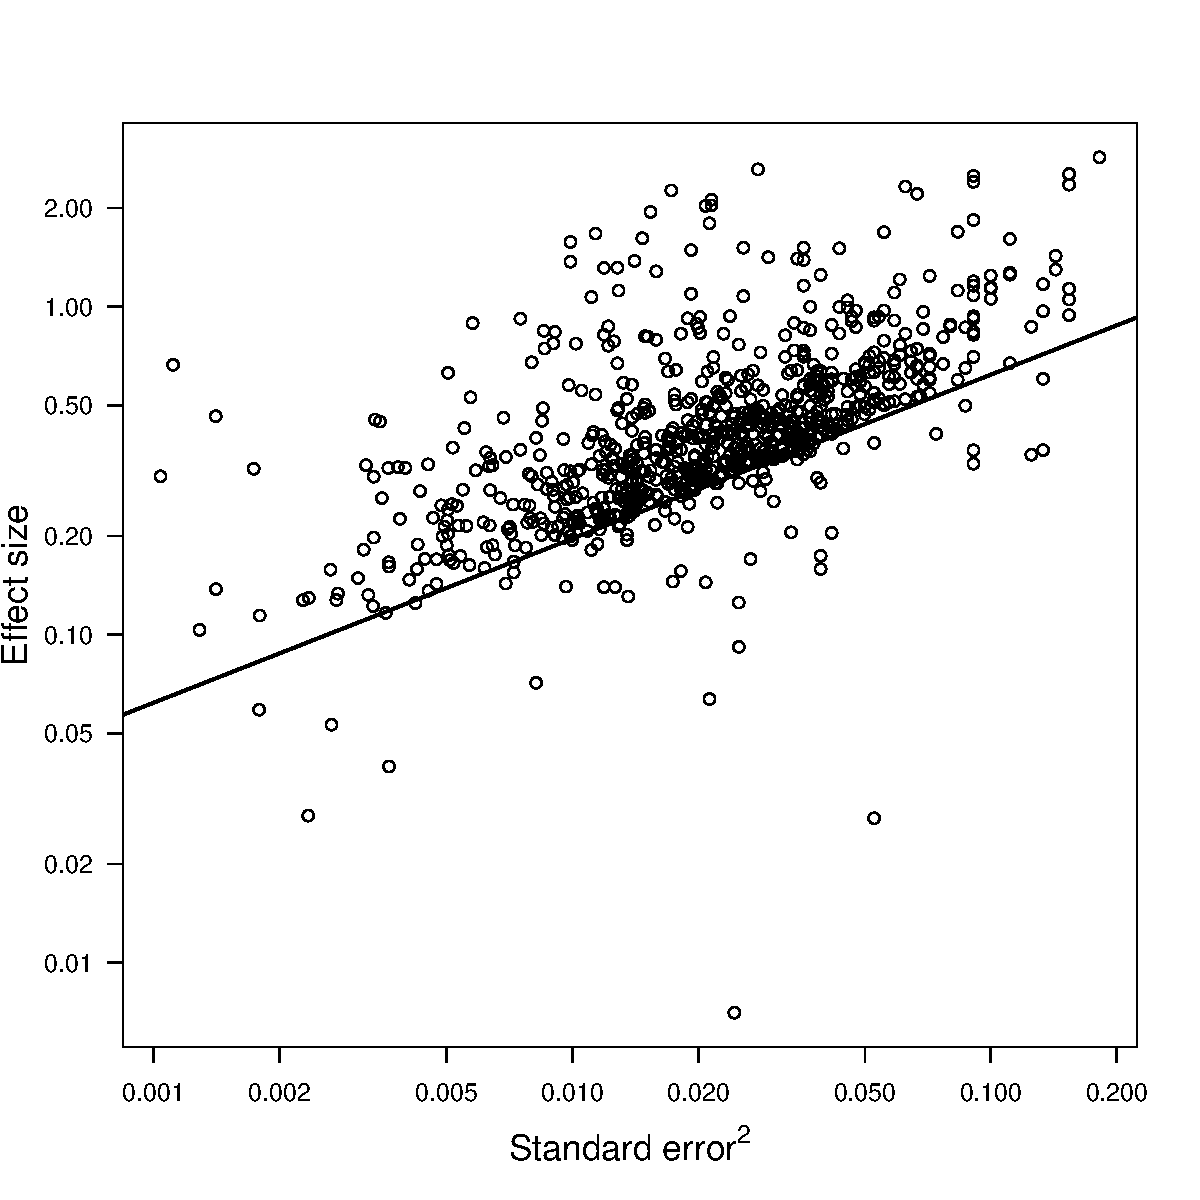
\includegraphics[scale=0.5]{chunks/motyl}
\par\end{centering}
\caption{\label{fig:motyl}Estimated effect sizes and squared standard errors
from \cite{Motyl2017-dx}. The black line is $y=1.96/\sqrt{n}$,
the treshold for significance using the two-sided normal \emph{p}-value.
Both axes are logarithmic. The number of studies is $n=862$, and
the percentage significant results is $91.5\%$.}
\end{figure}


\subsubsection{Correction for publication bias and $p$-hacking}

There are several methods that attempts to identify and even correct
for publication bias. The most widely used is the \emph{funnel plot}
of \cite{Egger1998-kj}, where the standard error of each study
is plotted against its effect size. Under severe publication bias,
this plot will be skewed. This is because small studies, which will
typically be those with high standard errors, must have large estimated
effect sizes in order to cross the $p=0.05$ boundary. An example
of such a plot is found in figure 2.1.

\begin{figure}
\noindent \begin{centering}
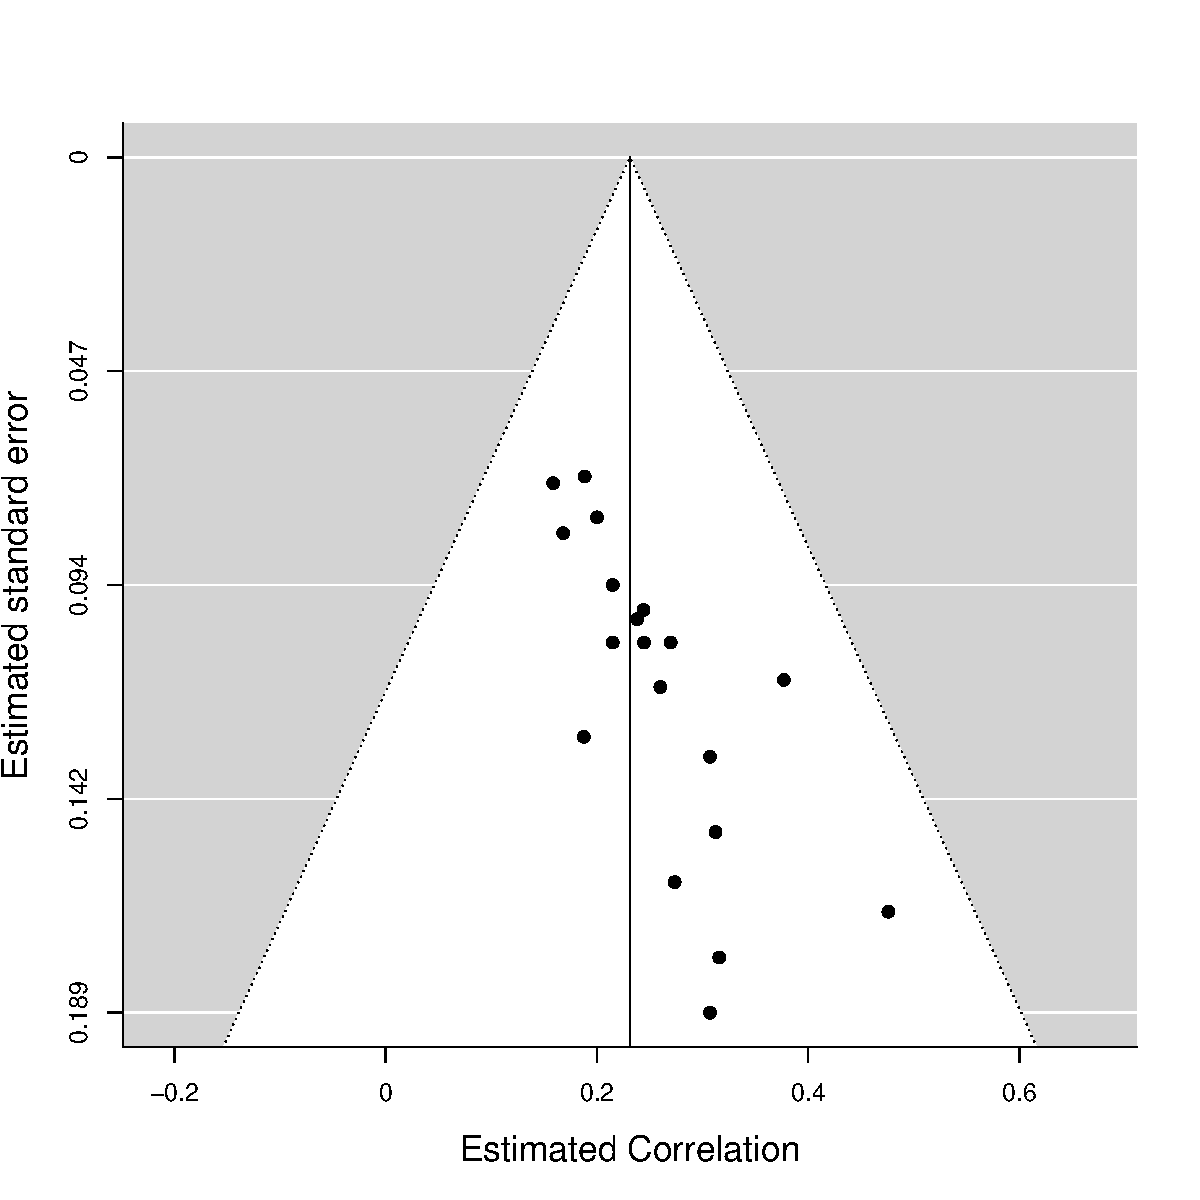
\includegraphics[scale=0.5]{chunks/anderson}
\par\end{centering}
\caption{\label{fig:A-funnel-plot}A funnel plot of a subset from the meta-analysis
of \cite{anderson_violent_2010} on the effect of violent video games
on aggressive behavior. The funnel plot is highly skewed to the left,
which indicates severe publication bias. The funnel plot was made
with the $\mathtt{R}$-package \cite{team_r_2000}
$\mathtt{metafor}$ \parencite{viechtbauer_conducting_2010}.}
\end{figure}

Under severe publication bias, this plot will be skewed. Building
on this method intuition, the authors propose to estimate a publication
bias-corrected effect size by running the regression
\[
z_{i}\sim\theta+\beta\widehat{s}_{i}+\epsilon_{i},
\]
where $\theta$ is the adjusted effect size and $\beta\neq0$ indicates
the presence publication bias This method is called PET \parencite{stanley_beyond_2005}.
But PET is not the only regression-based method for publication bias
correction. Another popular method is PET-PEESE \parencite{Stanley2014-gx},
a modified version of the above, applied mostly in economics research
and recently to psychology \parencite{carter_series_2015}. This method
is not without critics. \cite{gervais_putting_2015} claims the method
systematically underestimates the effect size in presence of publication
bias, making almost any effect appear to be indistinguishable from
$0$. In addition, \cite{simonsohn_[59]_2017} runs simulations to
show that the method fails in presence of inter-study heterogeneity.
The most popular method in medicine is named trim and fill \parencite{Duval2000-ct},
which is based on removing and adding non-observed studies to the
funnel plot in order to make it symmetric. The $p$-curve of \cite{simonsohn_p-curve:_2014}
has proven popular in psychology. This method is based on the theoretical
shape (under the null of no $p$-hacking) of the probability density
function obtained from the $p$-values from a set of studies. For
a simulation study comparing methods to account for publication bias,
see \cite{moreno_assessment_2009}.

All these methods share a serious shortcoming. Popular statistical
methods, such as linear regression and logistic regression, are based
on\emph{ explicitly defined models}. These models allows for clear
cut estimation of parameters, parameters with univocal definitions
and interpretations. The methods for publication bias are not based
on explicit models. As such, their estimated quantities are hard to
interpret, and are defined in an offhand way. For instance, PET-PEESE
is based on one half intuition, one half semi-rigorous mathematics;
the $p$-curve of is based on statistical properties of a null-model
we assume that is false. While there are several statistical methods
used to model heterogeneity, as discussed in the previous chapter,
none of them have been directly extended to take publication bias.
The product of this flaw is that all corrections for publication bias
are \emph{ad hoc}, which partially explain their poor performance. 

The meta-analyst will have to make a choice of correcting for publication
bias or not. If she opts to correct for publication bias, she is faced
with a large number of different methods, none of them particularly
good, but if her choice is no, her resulting estimates might be severely
biased. The effect of this choice is potentially tremendous. As an
illustration, I take a well-known contentious issue from economics:
What is the relationship between the minimum wage and employment?
The predictions from economic theory about this are unequivocal: Rising
the minimum wage should raise the rate of unemployment. There are
two reasons why: First, when the minimum wage is raised above the
competitive wage, the employer will shift his spending towards other
venues such as capital investments. Second, the industries affected
will increase their prices to consumers, reducing the demand for labor
in turn. \cite{doucouliagos_publication_2009} studies the empirical
research the relationship between a minimum wage floor and employment.
Their meta-analysis contains $64$ studies, which in turn contain
a total of $1474$ employment elasticity estimates. The average elasticity
was $-0.19$, while the fixed effects meta-analytic estimate was $-0.054$,
both highly significant. However, their publication bias-corrected
estimate was the meager $-0.01$. In the words of \cite{doucouliagos_publication_2009}:
``An elasticity of -0.01 has no meaningful policy implications. If
correct, the minimum wage could be doubled and cause only a 1 per
cent decrease in teenage employment.'' In this case the decision
to correct for publication bias reduced the effect size estimate with
a factor of $5$. Needless to say, this could have huge policy implication,
recall the recent push towards rising the minimum wage in California
and other U.S. states.

Since publication bias and $p$-hacking is ubiquitous and its effect
can make the difference between two radically different conclusions,
good methods for dealing with it is needed. Since the current methods
do not live up to the task, research on improving these methods are
needed. Even more important, scientist should rigorous in their usage
of methods designed to avoid publication bias and $p$-hacking, for
instance study pre-registration. 

\subsection{Back-of-the-envelope calculations }

A large part the daily lives of researchers is spent in reading and
critically engaging with other peoples research. Prior to the replication
crisis, a common way to judge the worth of an effect was to look at
its \emph{p}-value or \emph{t-}value. If the \emph{p}-value was smaller
than $0.05$, or the \emph{t-}value larger than approximately $2$,
results looked impressive enough to be worthy of consideration. While
plenty of researchers believe this way to do consume research is bad
\parencite{Gigerenzer2004-oc}, it is not without its mertis. We have
limited attention span and need to abide by some decision rules; what
we need are justified decision rules that will not lead us astray
with an unacceptably high probability.

Making some half-plausible assumptions, there is simple a way to correct
effect sizes for publication bias and \emph{p}-hacking. This back-of-the-envelope
method is based on a simple model of selection for significance, where
we observe only significant normal $X$s. Assume $X\sim N(\mu,n^{-1/2})$
and let $U=\Phi(-n^{1/2}X)$ be the standard one-sided $p$-value.
The expectation of the left-truncated normal is \parencite[Section 10.1]{Johnson1994-ag}

\begin{equation}
\mu+\sigma M'\left(\frac{a-\mu}{\sigma}\right).\label{eq:mean of truncated normal}
\end{equation}
In our case, $a=c_{\alpha}n^{-1/2}$ and $\sigma=n^{-1/2},$ and the
expectation equals $\mu+n^{-1/2}M'(c_{\alpha}-n^{1/2}\mu)$. When
$\mu=0$ and $\alpha=0.05$, get $E(X\mid n^{1/2}X>c_{\alpha})=n^{-1/2}\alpha^{-1}\phi(c_{\alpha})\approx2n^{-1/2}.$
This value is easy to remember and compute, and provides a realistic
baseline to compare effect sizes against. In a world free of biases,
we would informally compare an effect size against $0$. In a world
with publication bias and \emph{p}-hacking, comparing against $2n^{-1/2}$
smarter and almost as easy. From the data set of \cite{Motyl2017-dx}
we just looked at, we get $2\overline{n^{-1/2}}=0.24$. That is, we
would expect a mean effect size of $0.24$ from psychology even when
the true mean is $0$, assuming complete selection for significance
and the validity of the normal approximation. The actual mean of the
data set, $\overline{\theta}=0.45$, does not look that impressive
anymore.

There are strong reasons to care not only about \emph{p}-values, but
also about effect sizes \parencite{Funder2019-tg}. The natural way to
estimate $\mu$ is to use the maximum likelihood estimator $\hat{\mu}$.
While this quantity is easy to calculate numerically, it is hardly
convenient to use when reading a paper. Luckily, there are simple
bounds for the maximum likelihood estimator.
\begin{proposition}
\label{prop:maximum likelihood bounds}The maximum likelihood estimator
of $d$, called $\hat{d}$, based on a single observation $x$ from
a study with $n$ participants is bounded by 
\[
l(x)\leq\hat{d}(x)\leq u(x).
\]
The bounds are equal to
\begin{eqnarray}
l(x) & = & x-\frac{1}{n^{1/2}\delta},\label{eq:lower bound}\\
u(x) & = & x-\frac{1}{n^{1/2}\delta}\max\{1-\delta^{2},0\}.\label{eq:upper bound}
\end{eqnarray}
where $\delta=n^{1/2}x-\Phi^{-1}(1-\alpha)$.
\end{proposition}
Proposition \pageref{prop:maximum likelihood bounds} is a straight-forward
corollary of the following propositon. 
\begin{proposition}
\label{prop:ml bouds}Let $X_{1},\ldots,X_{N}$ be independent samples
from a left-truncated normal. Assuming known truncation point $a$
and standard deviation $\sigma$, the maximum likelihood estimator
$\hat{\mu}$ of $\mu$ is bounded by
\begin{equation}
\overline{x}-\frac{\sigma^{2}}{\overline{x}-a}<\hat{\mu}<\overline{x}-\max\left(\frac{\sigma^{2}}{\overline{x}-a}-(\overline{x}-a),0\right).\label{eq:ml bounds}
\end{equation}
\end{proposition}
\begin{proof}
Differentiating the logarithm of the density of a truncated normal,
we find that the maximum likelihood estimator is the solution to $\mu=\overline{x}-\sigma M'([a-\mu]/\sigma),$where
$M'(\text{\ensuremath{\theta}})=\phi(\text{\ensuremath{\theta}})/\Phi(-\text{\ensuremath{\theta}})$
is the inverse Mills' ratio. The inverse Mills' ratio can be bounded
elementary functions \parencite{Yang2015-pa}. In particular, it can be
bounded by \parencite[Equation 32]{Gasull2014-hn}
\begin{equation}
M_{u}(\theta)=\frac{1}{2}(\sqrt{\text{\ensuremath{\theta}}^{2}+4}+\text{\ensuremath{\theta}})>M'(\text{\ensuremath{\theta}}),\label{eq:Mills' ratio inequality}
\end{equation}
and 
\begin{equation}
M'(\text{\ensuremath{\theta}})>\frac{1}{4}(\sqrt{\text{\ensuremath{\theta}}^{2}+8}+3\text{\ensuremath{\theta}})=M_{l}(\theta)>\theta.\label{eq:Mill's ratio inequality (2)}
\end{equation}
The functions $M(\text{\ensuremath{\theta}})$ in these inequalities
are increasing in $\text{\ensuremath{\theta}}$, hence $\overline{x}-\sigma M([a-\mu]/\sigma)$
is icreasing in $\mu$. Assume $\mu_{u}$ satisfies $\mu_{u}=\overline{x}-\sigma M_{u}([a-\mu_{u}]/\sigma)$.
Since $M_{u}(\theta)>M'(\theta)$, we have $\overline{x}-\sigma M'([a-\mu_{u}]/\sigma)<0$
too, thus $\mu_{u}<\hat{\mu}$. Likewise, if $\mu_{l}$ satisfies
$\mu_{l}=\overline{x}-\sigma M_{l}([a-\mu_{l}]/\sigma)$, then $\mu_{l}>\hat{\mu}$.
Now define $l(\overline{x})=\mu_{u}$ and $u(\overline{x})=\mu_{l}$.
Now, to find $l(\overline{x})$, solve
\[
\mu=\overline{x}-\sigma\frac{1}{2}(\sqrt{\text{\ensuremath{([a-\mu]/\sigma)}}^{2}+4}+\text{\ensuremath{[a-\mu]/\sigma}})
\]
to get $\mu=\overline{x}-\sigma^{2}/(\overline{x}-a)$. The upper
bound $u(\overline{x})$ can be found in the same manner, using both
the lower bounds $M_{l}(\theta)$ and $\theta$ and choosing the best
option.
\end{proof}